\documentclass{article}
\usepackage[margin=2cm]{geometry}
\usepackage[pdftex]{graphicx}
\usepackage{algorithm}
\usepackage{algorithmic}
\renewcommand{\algorithmiccomment}[1]{//#1}
\begin{document}
\title{Learning to Play Atari Games}
\author{Matthew Hausknecht and Piyush Khandelwal}

\maketitle

\begin{abstract}
In this work we apply HyperNeat to the problem of learning how to play Atari games. By leveraging the geometric regularities present in the Atari game screen, HyperNeat is able to effectively evolve policies for playing several different Atari games. Results show that Hyperneat outperforms related RL and search techniques.
\end{abstract}

\section{Introduction}
Games have long been considered a fruitful domain for the study of AI. Seminal work on game playing includes Samuel's checkers playing program\cite{samuel_59} and Tesauro's TD-Gammon\cite{tesauro_94}. Games represent problems challenging enough to interest people yet abstract enough to be captured and modeled inside of computer programs. 

Common amoung many games is a representation of physical space. Board games as well as Atari games generally employ a 2-D overhead representation, with objects or pieces occupying distinct regions of space. Additionally, the dynamics of a given game, that is the movements and interactions of pieces, are often independent of the absolute locations. That is to say, when moving a knight in chess, the relative movement remains constant regardless of the absolute position. This suggests that it may be an easier problem to learn to the dynamics of a game and then reuse these dynamics across the space of the board than to relearn the dynamics of the game at each possible position. In other words, we hope to exploit the geometric regularities in many domains in order to simplify the learning task.

\section{Background and Related Work}
%% ALE and naddaf
Previous work on Atari games includes a masters thesis by Yavar Naddaf\cite{naddaf10} at the University of Alberta. Modifying the popular Atari 2600 emulator, Stella, Naddaf quantifies the performance of several classes of learning agents on 50 different Atari games. Learning agents include variant of a Reinforcement Learning and search tree based methods. Our work builds on his existing framework by introducing a new class of learning agent -- a Hyperneat CPPN Learner. 

%% BEV and keepaway
Learning to play games based on overhead representations has been previously attempted by Verbansics and Stanley\cite{verbancsics10} who focused on the RoboCup Keepaway Soccer domain, a task in which some number of \"keeper\" agents must maneuver and pass a soccer ball so that it is not captured by one of the \"taker\" agents. Verbansics encodes the state of the game using an overhead representation of the objects on the playing field -- namely the keepers, takers, and the ball. In order to exploit the geometric regularities present in this \"Bird's Eye View\" of the field, employs HyperNeat to learn a policy for playing this game. Results show that the learned policy is competitive with top learning algorithms for this task. Additionally, it is demonstrated that the learned policy can be transferred with no further learning to the same task at higher resolution or a different number of players on the field. This is a result of the indirect encoding present in the HyperNeat CPPN. 

Previously HyperNEAT has been successfully applied to other domains such as checkers\cite{gauci08}, multi-agent predator prey\cite{ambrosio08}, and quadruped locomotion\cite{clune09}. 

We apply the learning algorithm in Verbansics' work (HyperNeat) to a new domain -- that of Atari games. In many ways Atari games are more challenging RoboCup Keepaway. For example, while there is a fixed number of object classes in the game of keepaway (eg takers, keepers, and ball), each different Atari game may contain an arbitrary number of classes of objects which interact with each other in unexpected ways. 

\section{HyperNeat}
In this section we review the fundamentals of the HyperNeat learning algorithm. Hypercube-NEAT (HyperNeat) in an extension of the Neuro Evolution of Augmenting Topologies (NEAT) algorithm\cite{stanley02}. HyperNEAT, introduced by Gauci and Stanely\cite{gauci08}, evolves an indirect encoding or compressed description of a solution network. For example, while NEAT will evolve the topology and weights of a neural network which is then used to directly compute the solution to a problem, HyperNEAT evolves the topology and weights of a Compositional Pattern Producing Network (CPPN) which is used to determine the weights of the solution network. In this way, HyperNEAT is able to learn the geometric relationships of a domain through an indirect encoding that describes how the connectivity of an Artificial Neural Network (ANN) can be generated as a function of domain geometry. 

Specifically, HyperNEAT evolves the topology and weights of a CPPN. A CPPN is identical to an ANN except that rather than computing the target function of a task, a CPPN computes the weights of a corresponding ANN which then computes the target function. Figure \ref{fig:cppn} shows a graphical depiction of the relationship between a CPPN and its corresponding ANN. Because connection weights are produced as a function of a pair nodes in the substrate (ANN) whose geometric relationship is known, geometric knowledge may be encoded into the ANN. 

\begin{figure}[htp]
\begin{center}
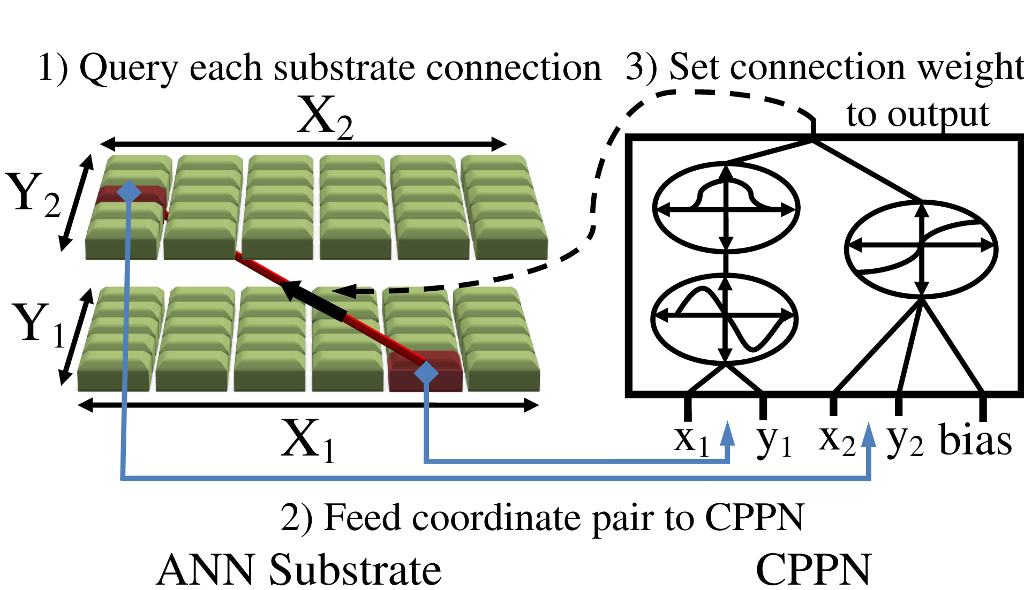
\includegraphics[scale=.3]{figures/cppn.png}
\end{center}
\caption{An fully connected ANN (left) is used to compute the target function for a task. The weights between each pair of substrate nodes are determined by the CPPN (right). The CPPN is itself an ANN which takes as input the locations of the pair of nodes whose connection weight is being determined and computes as output the weight of that connection. Before the ANN (left) can be used to compute the target function, each pair of nodes must have their corresponding connection weight determined.}
\label{fig:cppn}
\end{figure}

\section{Approach}

In this section we describe the details of our approach -- the main points are the manner in which the raw Atari game screen is processed to form an overhead representation amenable to HyperNEAT and the condor framework used to parallelize and speedup the evaluation of individuals.

\subsection{Visual Processing}

For nearly any machine learning problem, the question of how to encode the state space is of great importance. Following Verbansics' example, we seek an overhead representation of the game screen which includes relevant objects. While in the Keepaway domain, the set of relevant objects is somewhat apparent, as it may also be for any given Atari game, we need a way of identifying relevant objects across a large set of possible Atari games.

To answer the need, we design a simple visual processing stack which identifies objects and game entities without a priori knowledge of the specific game. A graphical depiction of this stack is shown in Figure \ref{fig:visproc}.

\begin{figure}[htp]
\begin{center}
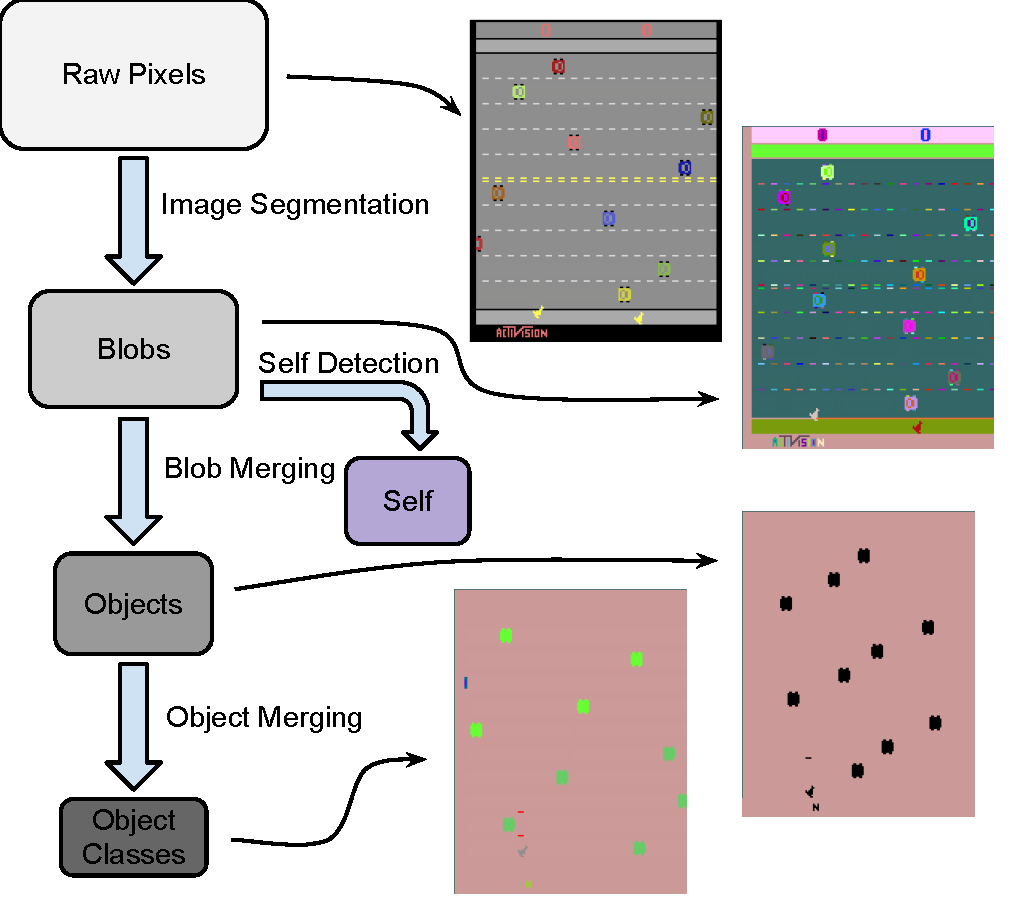
\includegraphics[scale=.8]{figures/AtariArch}
\end{center}
\caption{Visual Processing Architecture. Filled arrows denote the processing steps. Narrow arrows show examples of the game screen after each processing step for the game Freeway. The results of the Self Detection step are shown in gray on the Object Classes screen capture in which the algorithm has successfully identified the chicken as Self.}
\label{fig:visproc}
\end{figure}

Visual processing begins at the raw pixels of the game screen. Image Segmentation is performed at the first layer of stack in which adjacent raw pixels with similar colors are combined to form blobs. At the next level blob merging occurs which outputs a set of current objects on screen. The process of blob merging examines all of the recently discovered blobs in order to identify adjacent blobs which have the same velocity. These adjacent blobs are then merged into an object. (Velocity of blobs is computed by matching each blob with its counterpart in the previous frame and calculating displacement based on the centroids of the two blobs). Finally, similar objects are merged into object classes. In order to do this, the shape of each pair of objects is compared and if found to exceed a threshold (97\% pixel match in these experiments), the objects were said to belong to the same class. As the object class image in Figure \ref{fig:visproc} indicates, different object classes were discovered for the cars at the bottom half of the screen (light green), cars at the top half of the screen (dark green -- cars at top and bottom show slight differences as they are mirror images of each other), chicken (gray), and lane separators (red). It is assumed here that objects belong to the same class if their shape is relatively similar. This could be a false assumption in certain games where objects may look similar but interact differently -- however we have yet to encounter such a game.

\subsection{Self Identification}
The self detection step is meant to identify the location of entity which is being controlled. In the vast majority of Atari games, when actions are taken, they affect the movement of some entity on screen that is being controlled by the player. We hypothesize that identifying this entity that is being controlled would serve as a useful piece of information for a learning algorithm like HyperNEAT. (There are some notable exceptions in which no such self exists, but they are few and far between.) The self identification algorithm is based on information gain. The pseudocode for the algorithm is given in Algorithm \ref{alg:idself}.

\begin{algorithm}
\caption{Identify Self}
\label{alg:idself}
\begin{algorithmic}
  \STATE $possible\_actions \leftarrow $ set of actions applicable to this game
  \STATE $current\_blobs \leftarrow $ set of blobs in the current game frame
  \STATE $ActionHistory \leftarrow \{a_0...a_n\}$ \COMMENT{Actions at time 0...n}
  \FOR{blob $b \in current\_blobs$}
  \STATE $vHistory_b \leftarrow \{v_0...v_n\}$ \COMMENT{Velocity of blob $b$ at each timestep in the history}
  \STATE $H_b \leftarrow H(vHistory)}$ \COMMENT{Information entropy of $b$'s velocity history}
  \FOR{action $a \in possible\_actions$}
  \STATE $vHistory_{(b|a)} \leftarrow \{vHistory_b[t] ~\forall_t: ActionHist[t] == a\}$ \COMMENT{set of $b$'s velocities for timesteps in which action $a$ was taken}
  \STATE $H_{(b|a)} \leftarrow H(vHistory_{(b|a)})}$ \COMMENT{Information entropy of $b$'s velocity history given action $a$ was taken}
  \ENDFOR
  \STATE $InfoGain_b \leftarrow H_b - sum(p_a * H_{(b|a)})$ \COMMENT{$p_a$ is probability of action $a$ based on observed frequency} 
  \ENDFOR
  \RETURN $arg\_max_{b \in current\_blobs}(InfoGain_b)$ \COMMENT{Return blob with max information gain}
\end{algorithmic}
\end{algorithm}

At a high level, we assume there is a blob on screen which corresponds to the self. Additionally, we expect that this blob will move similarly whenever the same action is performed -- that is, whenever an action (Joystick Up) is taken, we expect the velocity of the self blob to have a similar value (blob y velocity = -1). Intuitively, assuming that random actions are taken, we expect the self blob to have a relatively high entropy taken over its full velocity history (since it should be going in random directions). However, we expect low entropy when taken over it's selective history conditioned on a specific action (since every time action up is taken the resulting velocity is -1). This should be true over all actions. Since information gain of a blob is defined as the information entropy of its full velocity history minus the weighted sum of selective velocity histories, we expect the self blob to exhibit maximum information gain. 

While this algorithm is generally successful in identifying the self blob, it has occasional problems with dynamics of certain environments. For example, in the Freeway game, after colliding with a car, the chicken (self blob) control is taken from the player and the chicken inadvertently moves down for several frames. The algorithm presented above has no way to know or account for periods of time in which the agent is out of the player's control and thus returns incorrect solutions when this is the case. 

\subsection{Condor Parallel Processing Framework}
This one is yours piyush.

\section{Results}

\section{Future Work}
There are many avenues of future work to explore. In general, we wish to extend the system presented here to work on a general and previously unknown games. One of the foremost difficulties we identified is dealing with multiple classes of objects. When providing input to the lowest substrate level in the HyperNEAT ANN, a floating point value much be provided for each substrate node. In Freeway, like in Robocup Keepaway, this is easily accomplished because there are only 2 different classes of objects -- cars and self for Freeway and takers and keepers for keepaway. This allows for an easy mapping from objects to substrate values -- for example, we assigned cars substrate values of -1 in order to encourage the agent to avoid them and gave the self a value of 1.0. In Keepaway, a similar thing is done in which takers get negative substrate values and keepers are given positives ones. 

This process of assigning values grows more complicated when there are more classes of objects on screen -- in the worst case a new game could have an arbitrarily large number of object classes. Furthermore, since visual processing is done on the fly during the course of the game, it is quite possible that new object classes may arise well after the start of the game. We have yet to clearly understand how well HyperNEAT is able to differentiate between classes of objects which are given very similar values when fed into the substrate (as is necessary when there are many different classes of objects). Another possible approach is to create multiple layers of input substrate -- one layer for each class of objects. We have yet to try this, but expect it would incur additional computational costs associated with a more complex ANN.

Another area of future work is finding a better way to handle the variable number of actions which may be present in different games. In games like Freeway where there are only 3 actions (up, down, noop) we can choose which action to take by comparing the value of the substrate node directly at, above, or below the self blob and taking the action corresponding to the maximally valued node. This becomes more complicated when other actions such as fire are included (it's not clear which node's value should be looked at to decide if the agent should fire). To address this issue, we believe that it may be possible to add another output layer to our substrate. This output layer would have a single node for each of the possible actions in the game and would simply take the action whose 3rd layer output node had the highest value. Figure \ref{fig:possiblearch} shows a graphical depiction of this alternative architecture.

\begin{figure}[htp]
\begin{center}
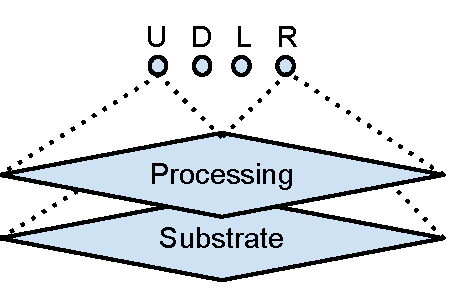
\includegraphics[scale=1]{figures/possiblearch}
\end{center}
\caption{Alternative architecture for handling variable numbers of actions. Assume full connectivity between levels (sparse connectivity shown with dotted arrows). This differs from the current architecture in that instead of choosing the agent's action based on values of nodes in the processing layer, we condense the processing layer into a third layer with an explicit node for each applicable action (U,D,L,R are example nodes corresponding to the actions Up, Down, Left, and Right).}
\label{fig:possiblearch}
\end{figure}

If the framework can be modified to handle the challenges of multiple object classes and variable numbers of actions, it should be general enough to tackle novel games without manual reconfiguration.

\section{Conclusion}


\bibliographystyle{plain}	
\bibliography{report}
\end{document}









